\documentclass[12pt, aspectratio=169]{beamer} % aspectratio = either 43 or 169
\usepackage[utf8]{inputenc}
\usepackage{graphicx}
\usepackage[T1]{fontenc}
\graphicspath{ {./img/} }

\usetheme{Hannover}
\mode<presentation>

% title and author
\title{Desplegando la R-API con Ansible}
\author{Luis Palomero}
\date{2021-04-23}
% document
\begin{document}


\frame{\titlepage}


\begin{frame}{Overview}
\tableofcontents
\end{frame}

\section{La R-API}
\subsection{Sobre la R-API}
\begin{frame}{La R-API}{La idea}

  \begin{block}{¿Qué es la R-API y qué objetivo tiene?}
    \begin{itemize}
    \item R-Api es un componente privado de la arquitectura de Declarando.
    \item Está parcialmente desacoplado.
    \item Ofrece capacidad de cómputo y resolución de problemas matemáticos/estadísticos.
    \end{itemize}
  \end{block}

\end{frame}

\begin{frame}{La R-API}{Estructura y componentes}
  Actualmente la R-API está formada por dos grandes componentes y un tercer componentes menor:
  \begin{itemize}
  \item Servidor reverso \textit{Nginx}: Capa de seguridad.
  \item Servidor R \textit{R-API}: Capa de aplicación completa.
    \item Package R \textit{Cashflow}: Package especializado.
    
  \end{itemize}
  
\end{frame}



\begin{frame}{La R-API}{Estructura y componentes}
  \begin{figure}
    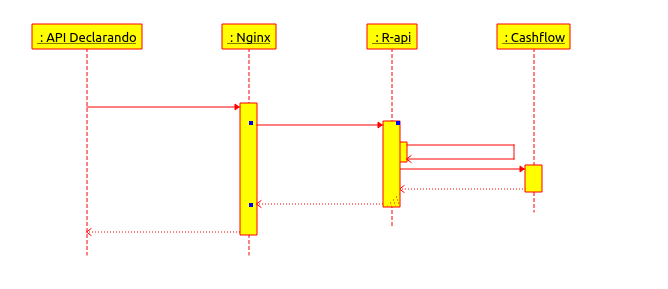
\includegraphics[width=1\textwidth]{20210407_1_estructura_clases.png}
    \label{fig:estructura_clases}
  \end{figure}

\end{frame}

\subsection{Componentes}

\begin{frame}{Componentes \textit{hardware}}
  Se ha creado una instancia que aloja la R-API de forma exclusiva. Esta instancia alberga una capa de Docker con los dos contenedores \textit{proxy\_server} y \textit{api} corriendo a la vez.

  Al estar en un servidor externo, se puede escalar la máquina según necesidad.

  Únicamente se puede acceder al servicio de \textit{api} a través del puerto 80 del proxy server\footnote{O así debería ser.}.

  \begin{figure}
    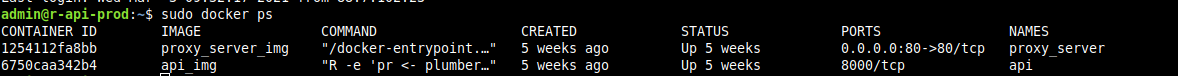
\includegraphics[width=1\textwidth]{20210407_2_docker.png}
    \label{fig:docker}
  \end{figure}

\end{frame}

\begin{frame}{Componentes \textit{hardware}}
  A nivel de comunicación externa de la instancia, se ha limitado el acceso a la misma fuera del bucle interno de red de Google.
  \begin{figure}
    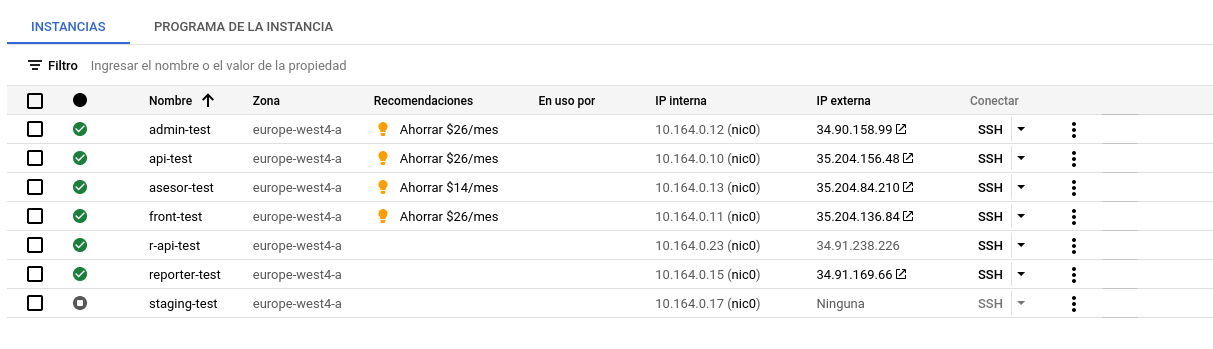
\includegraphics[width=1\textwidth]{20210407_3_servers.png}
    \label{fig:servers}
  \end{figure}
\end{frame}



\begin{frame}{Componentes software}{Repositorios}

\begin{itemize}
\item \textbf{Secure-r-api-base}: Base sobre la que se construye la imagen R-API. Almacena componentes y librerías.
\item \textbf{Secure-R-API} 
  \begin{itemize}
    \item Servidor reverso \textbf{NGINX} que nos añade una capa de seguridad.
    \item Servidor \textbf{R-Plumber}, sobre el que se ejecuta el código fuente de la R-API.
  \end{itemize}
\item \textbf{Cashflow}: Código de soporte que realiza predicciones de flujo de caja.
\end{itemize}
\end{frame}




\subsection{El problema del despliegue de la R-API}

\begin{frame}{Objetivo y restricciones}
  \begin{itemize}
  \item Iterar rápido en las primeras versiones.
  \item Poder desplegar \textit{aquí y ahora}.
  \item No debemos depender de los despliegues del componente principal.
  \item Poder recrear la infraestructura de forma sencilla.
  \item \textbf{No} hacer cambios en caliente en las máquinas soporte.
  \end{itemize}
  
\end{frame}

\section{Ansible}

\begin{frame}{Overview}
\tableofcontents
\end{frame}


\subsection{Conociendo Ansible}

\begin{frame}{¿Qué es Ansible?}
  \begin{block}{Wikipedia:}
    Ansible es una plataforma de software libre para configurar y administrar ordenadores.
  \end{block}

  Es una herramienta de \textit{Red Hat} que en este caso nos permite simplificar la creación de las instancias de las máquinas soporte y hacer despliegues de forma sencilla.
\end{frame}

\begin{frame}{Comparando Ansible vs Bitbucket Pipelines}

\begin{table}[htbp]
\tiny
\begin{tabular}{|p{4cm}|p{3cm}|p{3cm}|}
\hline
 & \textbf{Ansible} & \textbf{BitBucket} \\ \hline
\textbf{¿Quién ejecuta el despliegue?} & Ordenador local del usuario & Servicio remoto \\ \hline
\textbf{Comunicación} & Command line local & Hooks de GIT \\ \hline
\textbf{Precio} & Gratuito & Pago por uso \\ \hline
\textbf{Configuración}  & YAML & YAML \\ \hline
\textbf{Seguridad / constraseñas} & Local & Variables de entorno remotas \\ \hline
\textbf{Caché} & Sí & No \\ \hline  
\textbf{Gestión de entornos} & Ficheros de entorno & Nombre de la rama/YAML \\ \hline
\end{tabular}
\label{}
\end{table}


\end{frame}

\subsection{Componentes}
\begin{frame}{Ansible Playbook}
  \begin{itemize}
  \item Ese la piedra angular de Ansible: El script de automatización de tareas.
  \item Se ejecuta en base a un fichero de configuración YAML.
  \item Integra la plantilla Jinja2: Sustitución de variables y ejecución de bucles.
  \item Operativa: Se conecta a la maquina remota y ejecuta \textit{desde allí} los diferentes pasos del YAML.
  \end{itemize}
\end{frame}

\begin{frame}{Ansible Vault}
  \begin{itemize}
  \item Es la capa de seguridad de Ansible.
  \item Permite codificar y decodificar cualquier fichero.
  \item Gracias a él podemos almacenar y versionar variables delicadas en el repositorio.
  \end{itemize}
\end{frame}

\section{Desplegando la R-API}

\begin{frame}{Overview}
\tableofcontents
\end{frame}


\subsection{Interactuando con Ansible}

\begin{frame}{Seguridad y constraseñas}
  Una de las ventajas de estar todo integrado es que se puede aprovechar la capa de seguridad que ofrece \textit{pass}. Se ha diseñado para que la contraseña maestra esté almacenada en el pass versionado y accesible a través del script \textit{vault-keyring-client.sh}

\end{frame}

\begin{frame}[fragile]{Ansible en local*}
El hecho que se pueda ejecutar en local permite integrarse con otras herramientas, como \textbf{Make}
\begin{verbatim}
deploy_test: 
  decrypt_declarando_certificate
  decrypt_credentials_test
  ansible-playbook \
     ./infra/ansible_playbooks/pb_deploy.yml -v \
     -e "@./environs/env_test.yml"  \
     -i ./infra/hosts \
     --vault-id ./infra/vault-keyring-client.sh
  rm /tmp/declarando.crt
  rm /tmp/declarando.key
\end{verbatim}
\end{frame}


\subsection{Levantando una instancia}
\begin{frame}[fragile]{Cómo levantar y provisionar una nueva instancia*}
\begin{verbatim}
make create_r_api_instance_test 
make provision_r_api_instance_test
\end{verbatim}
\end{frame}



\subsection{Desplegando nueva versión}
\begin{frame}[fragile]{Cómo desplegar una nueva versión*}
\begin{verbatim}
make deploy_test 
\end{verbatim}

  \begin{block}{¡¡Ojo!!}
    Este \textit{make} desplegará en test (o producción si es \textit{make deploy\_prod}) \textbf{el estado actual} del código, en otras palabras \textbf{Git NO} está involucrado en el proceso de despliegue.
  \end{block}

\end{frame}

\section{Conclusiones}

\begin{frame}{Overview}
\tableofcontents
\end{frame}

\begin{frame}{Conclusiones}
  \begin{itemize}
  \item La \textit{R-API} es un componente auxiliar que \textit{externaliza} capacidad de cómputo de R.
  \item \textit{Ansible} es una tecnología de software libre que permite hacer despliegues de forma:
    \begin{itemize}
    \item Desde el mismo computador.
    \item De forma automatizada y gratuita.
    \end{itemize}

  \end{itemize}
\end{frame}

\begin{frame}{}
  \centering \Large
  \emph{Muchas gracias, ¿preguntas?}
\end{frame}



\end{document}